
%(BEGIN_QUESTION)
% Copyright 2011, Tony R. Kuphaldt, released under the Creative Commons Attribution License (v 1.0)
% This means you may do almost anything with this work of mine, so long as you give me proper credit

This P\&ID shows an incinerator stack used to safely burn poisonous gases.  The high temperature of the gas flame reduces the poisonous compounds to relatively harmless water vapor, carbon dioxide, and oxides of sulfur and nitrogen.

The incinerator was recently out of service for three full weeks being rebuilt.  Following the rebuild, operations personnel have attempted to start the incinerator's burner on plant fuel gas with no success.  They can get it started with natural gas, but the burner management system keeps tripping whenever they switch to fuel gas.  They call you to investigate.

$$\includegraphics[width=15.5cm]{i0004rx01.eps}$$

\vfil \eject

Identify the likelihood of each specified fault in this process.  Consider each fault one at a time (i.e. no coincidental faults), determining whether or not each fault could independently account for {\it all} measurements and symptoms in this process.

% No blank lines allowed between lines of an \halign structure!
% I use comments (%) instead, so that TeX doesn't choke.

$$\vbox{\offinterlineskip
\halign{\strut
\vrule \quad\hfil # \ \hfil & 
\vrule \quad\hfil # \ \hfil & 
\vrule \quad\hfil # \ \hfil \vrule \cr
\noalign{\hrule}
%
% First row
{\bf Fault} & {\bf Possible} & {\bf Impossible} \cr
%
\noalign{\hrule}
%
% Another row
SV-115 leaking air &  &  \cr
%
\noalign{\hrule}
%
% Another row
PSL-105 failed &  &  \cr
%
\noalign{\hrule}
%
% Another row
PSL-114 failed &  &  \cr
%
\noalign{\hrule}
%
% Another row
PCV-39 pressure setpoint too low &  &  \cr
%
\noalign{\hrule}
%
% Another row
PCV-39 pressure setpoint too high &  &  \cr
%
\noalign{\hrule}
%
% Another row
PCV-40 pressure setpoint too low &  &  \cr
%
\noalign{\hrule}
%
% Another row
PCV-40 pressure setpoint too high &  &  \cr
%
\noalign{\hrule}
%
% Another row
ZS-38 failed &  &  \cr
%
\noalign{\hrule}
%
% Another row
Blind inserted in natural gas header &  &  \cr
%
\noalign{\hrule}
%
% Another row
Blind inserted in fuel gas header &  &  \cr
%
\noalign{\hrule}
} % End of \halign 
}$$ % End of \vbox

\underbar{file i03500}
%(END_QUESTION)





%(BEGIN_ANSWER)

% No blank lines allowed between lines of an \halign structure!
% I use comments (%) instead, so that TeX doesn't choke.

$$\vbox{\offinterlineskip
\halign{\strut
\vrule \quad\hfil # \ \hfil & 
\vrule \quad\hfil # \ \hfil & 
\vrule \quad\hfil # \ \hfil \vrule \cr
\noalign{\hrule}
%
% First row
{\bf Fault} & {\bf Possible} & {\bf Impossible} \cr
%
\noalign{\hrule}
%
% Another row
SV-115 leaking air &  & $\surd$ \cr
%
\noalign{\hrule}
%
% Another row
PSL-105 failed &  & $\surd$ \cr
%
\noalign{\hrule}
%
% Another row
PSL-114 failed &  & $\surd$ \cr
%
\noalign{\hrule}
%
% Another row
PCV-39 pressure setpoint too low &  & $\surd$ \cr
%
\noalign{\hrule}
%
% Another row
PCV-39 pressure setpoint too high &  & $\surd$ \cr
%
\noalign{\hrule}
%
% Another row
PCV-40 pressure setpoint too low & $\surd$ &  \cr
%
\noalign{\hrule}
%
% Another row
PCV-40 pressure setpoint too high & $\surd$ &  \cr
%
\noalign{\hrule}
%
% Another row
ZS-38 failed &  & $\surd$ \cr
%
\noalign{\hrule}
%
% Another row
Blind inserted in natural gas header &  & $\surd$ \cr
%
\noalign{\hrule}
%
% Another row
Blind inserted in fuel gas header & $\surd$ &  \cr
%
\noalign{\hrule}
} % End of \halign 
}$$ % End of \vbox

%(END_ANSWER)





%(BEGIN_NOTES)

\vskip 20pt \vbox{\hrule \hbox{\strut \vrule{} {\bf Virtual Troubleshooting} \vrule} \hrule}

This question is a good candidate for a ``Virtual Troubleshooting'' exercise.  Presenting the diagram to students, you first imagine in your own mind a particular fault in the system.  Then, you present one or more symptoms of that fault (something noticeable by an operator or other user of the system).  Students then propose various diagnostic tests to perform on this system to identify the nature and location of the fault, as though they were technicians trying to troubleshoot the problem.  Your job is to tell them what the result(s) would be for each of the proposed diagnostic tests, documenting those results where all the students can see.

During and after the exercise, it is good to ask students follow-up questions such as:

\begin{itemize}
\item{} What does the result of the last diagnostic test tell you about the fault?
\item{} Suppose the results of the last diagnostic test were different.  What then would that result tell you about the fault?
\item{} Is the last diagnostic test the best one we could do?
\item{} What would be the ideal order of tests, to diagnose the problem in as few steps as possible?
\end{itemize}

%INDEX% Basics, control loop troubleshooting (realistic P&ID shown)
%INDEX% Control, strategies: cascade (realistic P&ID shown)
%INDEX% Fieldbus, HART: multivariable instrument (realistic P&ID shown)
%INDEX% Process: incinerator (realistic P&ID shown)

%(END_NOTES)

